
%%%%%%%%%%%%%%%%%%%%%%% file typeinst.tex %%%%%%%%%%%%%%%%%%%%%%%%%
%
% This is the LaTeX source for the instructions to authors using
% the LaTeX document class 'llncs.cls' for contributions to
% the Lecture Notes in Computer Sciences series.
% http://www.springer.com/lncs       Springer Heidelberg 2006/05/04
%
% It may be used as a template for your own input - copy it
% to a new file with a new name and use it as the basis
% for your article.
%
% NB: the document class 'llncs' has its own and detailed documentation, see
% ftp://ftp.springer.de/data/pubftp/pub/tex/latex/llncs/latex2e/llncsdoc.pdf
%
%%%%%%%%%%%%%%%%%%%%%%%%%%%%%%%%%%%%%%%%%%%%%%%%%%%%%%%%%%%%%%%%%%%


\documentclass[runningheads,a4paper]{llncs}

\usepackage{amssymb}
\setcounter{tocdepth}{3}
\usepackage{graphicx}

\usepackage{balance}
\usepackage{lmodern}
\usepackage{tikz}
\usetikzlibrary{arrows,shadows,patterns}
\usepackage{pgf-umlsd}
%\usepgflibrary{arrows} % for pgf-umlsd
\usepackage{pgfplots}
\usepackage{pgfplotstable}
%\usepackage{amsmath}
%\usepackage{subcaption}
\usepackage[caption=false]{subfig}

\usepackage{dblfloatfix}

\usepackage{listings}

\usepackage{color}

\definecolor{red}{rgb}{1,0,0}
\definecolor{green}{rgb}{0,1,0}
\definecolor{blue}{rgb}{0,0,1}
\definecolor{cyan}{rgb}{0.4,1,1}
\definecolor{orange}{rgb}{1,0.7,0}
\definecolor{dkgreen}{rgb}{0,0.6,0}
\definecolor{gray}{rgb}{0.5,0.5,0.5}
\definecolor{purple}{rgb}{0.58,0,0.82}

\usepackage{url} 
\newcommand{\keywords}[1]{\par\addvspace\baselineskip
\noindent\keywordname\enspace\ignorespaces#1}

\newcommand{\hl}[1]{\textcolor{dkgreen}{#1}}
\newcommand{\fixme}[1]{\textcolor{red}{{\em TODO}: \bf #1}}

\begin{document}

\mainmatter  % start of an individual contribution

% first the title is needed
\title{Squirrel: Architecture Driven Resource Management}

% a short form should be given in case it is too long for the running head
\titlerunning{Squirrel: Architecture Driven Resource Management}

% the name(s) of the author(s) follow(s) next
\author{Inti Gonzalez-Herrera\inst{1}
\and Johann Bourcier\inst{1}
\and Walter Rudametkin\inst{2}
\and\\ Olivier Barais\inst{1}
\and Francois Fouquet\inst{3}}
%
\authorrunning{Squirrel: Architecture Driven Resource Management}
% (feature abused for this document to repeat the title also on left hand pages)

% the affiliations are given next; don't give your e-mail address
% unless you accept that it will be published
\institute{University of Rennes 1 - IRISA, 35042 Rennes, France,\\
\email{\{inti.glez,johann.bourcier,barais\}@irisa.fr},
\and
University of Lille - INRIA,
Cit\'{e} Scientifique Villeneuve d{'}Ascq, France\\
\email{walter.rudametkin@univ-lille1.fr},
\and
University of Luxembourg,
Luxembourg, Luxembourg,\\
\email{francois.fouquet@uni.lu}
}

%\toctitle{Lecture Notes in Computer Science}
%\tocauthor{Authors' Instructions}
\maketitle


\begin{abstract}
Resource management is critical to guarantee Quality of Service when various stakeholders share the execution environment, such as cloud or mobile environments.
In this context, providing management techniques compatible with standard practices, such as component models, is essential.
Resource management is often realized through monitoring techniques, while resource isolation uses virtual machines or containers (e.g., docker).
These techniques (i) impose varying levels of overhead depending on the managed resource, and (ii) are applied at different abstraction levels, such as processes, threads or objects.
Thus, mapping components to system-level abstractions in the presence of resource management requirements can lead to sub-optimal systems.

%We propose Squirrel, an approach to automatically tune component deployment and resource management in order to maintain a good balance between management overhead and the level of sharing.
We propose Squirrel, an approach to tune component deployment and resource management in order to reduce management overhead.
%In Squirrel, an architectural model annotated with resource requirements is used at runtime to guide the mapping of components to system abstractions with different resource management capabilities and overhead.
At runtime, Squirrel uses an architectural model annotated with resource requirements to guide the mapping of components to system abstractions, providing different resource management capabilities and overhead.
%To evaluate the approach, 
We present an implementation of Squirrel, using a Java component framework,
%for a Java-based component platform
and a set of experiments to validate its feasibility and overhead.
%\hl{The results show how the right mapping selection can reduce the performance impact and memory footprint.[NEEDS IMPROVEMENT]}
We show that choosing the right \textit{component-to-system} mappings at deployment-time reduces performance overhead and/or memory use.
%The results show (i) better performance than system deployed with full isolation among components and, (ii) only memory overhead in certain situations when comparing an application against its version running without resource management.
\keywords{resource management, components, architecture adaptation}
\end{abstract}

%\section{Introduction}\label{sec:introduction}
%Garbage collection-based memory management is a wide\-spread approach nowadays since
%it improves software quality and eases the development process.
%Nonetheless, memory-related issues are still relevant in languages/runtimes with
%garbage collectors because developers tend to fail during memory manipulation.
%In particular, it is known that memory leaks and unnecessary allocations are the sources
%of both functional and non-functional software misbehavior~\cite{cbse/14/attouchi/monitoring, Vera:2004:FAF:973097.973099}.

%Dealing with these issues have been a concern for both the industry and the academy
%for a while; therefore, there are several approaches to reduce the risk of memory-related
%errors.
%In the industry, practitioners use memory profilers (e.g. YourKit, Eclipse Memory
%Analyzer Tool and Plumbr) to deal with the problem.
%These tools support many sort of built-in analysis which are fairly efficient because
%they are based on industrial standards such as JVMTI.
%Some of them also provide mechanisms to specify user-defined analysis through a query 
%language such as OQL~\cite{OQL-visualvm}.
%Although useful, the usage of user-defined analysis requires in most cases the 
%generation of a costly heap dump which makes the associated queries unsuitable for
%at runtime execution in a production environment.
%Hence, it is not possible to use these tools to feed neither self-adaptive nor self-healing
%systems.

%In the academy, different approaches tackle memory issues~\cite{Xu:2015:MPP:2729552.2729565, Nguyen:2007:DEM:1296907.1296912, Bond:2008:TML:1449764.1449774, Jung:2014:AML:2568225.2568311}.
%Many of these solutions are either efficiently implemented as hard-coded modifications to the
%garbage collector or built on top of industrial standards as JVMTI.
%The advantage of these mechanisms is a reduction on the overhead of such analysis.
%However, they have two limitations: i) they target a single memory issue and ii) it is hard to
%introduce them in the industry.
%In general, implementing a highly efficient analysis requires knowledge of low-level APIs or
%garbage collection mechanisms which are not commonly in the curriculum of most managed runtime
%environment (MRE) users.

%It seems clear to us that there is a gap in existent solutions to analyze the heap.
%Either they are fairly {\em generic/easy to use} but offer poor performance or they offer good performance but are hard to customize/create. 
%We claim that a {\em simple to use} and efficient mechanism to perform memory analysis is
%a feature required in many areas of software development for MREs (e.g. to build self-adaptive systems, to
%reduce development complexity, to decrease the number of errors).  

%In this paper, we propose a framework to analyze the status of the memory heap and collect information about it.
%The main component of the framework is a domain-specific language (DSL) that allows us to specify
%how to explore and collect the desired information.
%The concepts of this language are highly coupled to the way the heap is traversed.
%A program in this language is compiled into a backing technology that support, in an efficient way, the iteration over all objects and 

%New software abstractions are created for good reasons, such as  having specific point of views on a particular system, simplifying software development, reducing errors, removing redundant tasks and improving productivity. 
%There is currently a trend in \glslink{SE}{SE} towards the creation of new languages and tools to support specific software developments~\cite{whittle2014state, van2000domain,hutchinson2011empirical}. 
%The design of such new languages and platforms are done for good reasons, such as  having specific point of views on a particular system, simplifying software development, reducing errors, removing redundant tasks and improving productivity. 
%This trend has led to the development of new research topics such as .
The \gls{SLE} community aims at reducing the effort required in engineering new languages and their corresponding development tools, thus improving the efficiency of both people in charge of designing new languages and their users~\cite{sle}. 
However, as far as we know, they do not take into account profiling tools, which are essentials for software maintenance and optimization.
Indeed, although specific tools are needed to monitor running systems in order to detect defects or abnormal behaviors~\cite{duesterwald2000software, Jovic:2011:CMY:2076021.2048081},
little support exists to ease their creation.

%Many of the newly designed languages and runtime platform are built on top of existing object oriented languages runtime such as the Java Virtual Machine (JVM). 
%Therefore people in charge of optimizing, debugging and maintaining software applications can use the existing debugger and profilers of these platforms. 
%However, there is a paradigm mismatch between the classical profilers used in object-oriented systems and the newly designed platforms and languages. 
%Indeed, the concepts introduced in these new languages may not exhibit a straightforward mapping to the underlying object-oriented system. For example, in the Spring framework~\cite{laddad2009aspectj}, some annotations like $@Aspect$ generate dynamic proxies on the fly. Existing profilers will present these proxies as normal objects, thus revealing a mismatch between the profiler and developer view. 

In this chapter, we focus on the problem of easing the creation of memory profilers for domain-specific software abstractions that are designed to be executed on top of MRTEs. 
We first propose a metalanguage to specific what data about the memory use is of interest in a domain (see Section~\ref{sec:approach}).
A profiler is then generated to collect the data and present it in terms of concepts of that language. 
In addition, we present a tooled DSL based on such a metalanguage, which generates profilers for the JVM (see Section~\ref{sec:implementation}).
%to match the language concepts and provide useful information to the end user.
An important point of our approach is the low overhead induced by these profilers; this makes them usable in production environments (see Sections~\ref{sec:expressiveness} and~\ref{sec:dsl-evaluation}).
%Indeed, generating a specific profiler from an abstract definition of the role of this profiler enable us to produce very specific profiler which only monitor the relevant information.

The contributions of this chapter are as follows:
\begin{itemize}
\item A metalanguage to describe what information a profiler must collect.
In addition, programs in this metalanguage also defines how to collect the information.
Although knowledge of the underline execution model is required, the procedure to obtain data is mostly defined without using low-level details.  

\item A concrete implementation of this metalanguage that target the JVM.
In particular, by using the \glslink{JVMTI}{JVMTI}, we are able to generate memory profilers with low overhead.
Concrete profilers already generated are portable to any implementation of the JVM that supports JVMTI.

\item A discussion of the metalanguage's expressiveness, and an evaluation of the performance overhead induced by three profilers in real-world use cases.
\end{itemize}

%The rest of this chapter is organized as follows
%A description of the DSL and its tooling support are presented in sections and .
%In section we discuss the expressiveness of the language.
% presents an evaluation of the performance achieved by the custom profilers.
%Related works are discussed in section~\ref{sec:relatedwork}.
%Finally, section~\ref{sec:conclusions} gives the conclusions and presents future works.

%\subsection{Copyright Forms}

%The copyright form may be downloaded from the ``For Authors"
%(Information for LNCS Authors) section of the LNCS Website:
%\texttt{www.springer.com/lncs}. Please send your signed copyright form
%to the Contact Volume Editor, either as a scanned pdf or by fax or by
%courier. One author may sign on behalf of all of the other authors of a
%particular paper. Digital signatures are acceptable.

\section{Background and motivating example}\label{sec:background}

%\subsection{Motivating example\label{sec:motivatingexample}}

%In this section we present a motivating example for the use of an optimistic adaptive monitoring process in the context of a real-time crisis management system in a fire department. 
During a dangerous event, many firefighters are present and need to collaborate to achieve common goals.
%In a situation where many firefighters are present and need to collaborate to handle a dangerous event, 
Firefighters have to coordinate among themselves and commanding officers need to have an accurate real-time view of the system.

The Daum project\footnote{\url{https://github.com/daumproject}} provides a software application that supports firefighters in these situations.
The application runs on devices with limited computational resources because it must be mobile and taken on-site.
%As the software have to be mobile to take it on site, it is running on devices with limited computation resources.
It provides numerous services for firefighters depending on their role in the crisis.
In this chapter, we focus on the two following roles:
\begin{itemize}
\leftskip -.2in
 \item A collaborative functionality that allows commanding officers to follow and edit tactical operations. The firefighters' equipment include communicating sensors that report on their current conditions.
 \item A drone control system which automatically launches a drone equipped with sensors and a camera to provide a different point-of-view on the current situation.
\end{itemize}

%\todo{I don't get this for example. It is not relate to the previous sentence.}For example, one service is related to firefighter information monitoring to know the location, activity and health status of each firefighter involved on the crisis but also to get some information on their environment (e.g. temperature, toxic gas). Another service is in charge of the management of victims. They must be redirected according to their needs.

As is common in many software applications, the firefighter application may have a potentially infinite number of configurations. These configurations depend on the number of firefighters involved, the type of crisis, the available devices and equipment, among other parameters. 
Thus, it is generally not possible to test all configurations to guarantee that the software will always function properly. 
Consequently, instead of testing all configurations, there is a need to monitor the software's execution to detect faulty behaviours and prevent system crashes. 
However, fine-grained monitoring of the application can have excessive overhead that makes it unsuitable with the application and the devices used in our example.
Thus, there is a need for an accurate monitoring system that can find faulty components while reducing overhead.

The Daum project has implemented the firefighter application using a Component Based Software Architecture.  The application makes extensive use of the Kevoree\footnote{\url{http://www.kevoree.org}\label{note:kevoree}} component model and runtime presented in chapter \ref{chap:abstractions_and_resource_management}.

% Using our adaptive monitoring solution, we are able to reduce the overhead of the monitoring process keeping enough well response time to find faulty behaviors.



\subsection{Kevoree}
Kevoree is an open-source dynamic component platform, which relies on Models@run.time~\cite{BlairBF09} to properly support the dynamic adaptation of distributed systems.
Our use case application and the implementation of the Scapegoat framework make extensive use of the Kevoree framework.
The following subsections detail the background on component-based software architecture, introduce the Models@run.time paradigm and give an overview of the Kevoree platform.

\subsubsection{Component-based software architecture}

Software architecture aims at reducing complexity through abstraction and separation of concerns by providing a common understanding of component, connector and configuration~\cite{xadl,Medvidovic:2000,VanOmmering-et-al-00}.
One of the benefits is that it facilitates the management of dynamic architectures, which becomes a primary concern in the Future Internet and Cyber-Physical Systems~\cite{DBLP:journals/ase/NittoGMPP08, Johnson:2015:CSM:2735960.2735979}.
Such systems demand techniques that let software react to changes by self-organizing its structure and self-adapting its behavior~\cite{PanzicaLaManna:2012:LDU:2304736.2304764, Johnson:2015:CSM:2735960.2735979, Zhang:2009:MVD:1509239.1509262}.
Many works~\cite{cbse-conference} have shown the benefits of using component-based approaches in such open-world environments~\cite{baresi2006toward, Caporuscio:2010:AIA:1985522.1985547, Perez-Palacin:2010:PAO:1712605.1712614}.

To satisfy the needs for adaptation, several component models provide solutions to dynamically reconfigure a software architecture through, for example, the deployment of new modules, the instantiation of new services, and the creation of new bindings between components~\cite{Porter:2014:RMC:2602458.2602471, Zheng:2014:RCC:2679601.2680405, Irmert:2008:RAS:1370018.1370036, Ghezzi:2010:QDD:2163764.2163774}. 
In practice, component-based (and/or service-based) platforms like Fractal~\cite{bruneton06}, OpenCOM~\cite{BlairCULJ04}, OSGi~\cite{OSGI:r5} or SCA~\cite{SEINTURIER:2011:INRIA-00567442:1} provide platform mechanisms to support dynamic architectures.

%As a result, component-based platforms offer a challenging playground for building adaptive monitoring framework as they raise a new challenge in easing the open-world paradigm and they can be an element of the solution. 

%In this context, traditional software development, based on the closed-world assumption that the  boundary between system and environment is known and unchanging does not work.


\subsubsection{Models@run.time}
Built on top of dynamic component frameworks, Models@run.time denote model-driven approaches that aim at taming the complexity of dynamic adaptation.
It basically pushes the idea of reflection~\cite{morin09a} one step further by considering the reflection-layer as a real model: ``something simpler, safer or cheaper than reality to avoid the complexity, danger and irreversibility of reality''.
In practice, component-based and service-based platforms offer reflection APIs that allow instrospecting the application (e.g., which components and bindings are currently in place in the system) and dynamic adaptation (e.g., changing the current components and bindings).
While some of these platforms offer rollback mechanisms to recover after an erroneous adaptation~\cite{leger2010reliable}, the purpose of Models@run.time is to prevent the system from actually enacting an erroneous adaptation. 
In other words, the ``model at runtime'' is a reflection model that can be decoupled from the application (for reasoning, validation, and simulation purposes) and then automatically resynchronized.
This model can not only manage the application's structural information (i.e., the architecture), but can also be populated with behavioural information from the specification or the runtime monitoring data.


\subsubsection{The Kevoree framework\label{sec:kevoree}}	
% Se proteger un peu plus sur Kevoree pour big node / placer plus de ref / comparaison ?
%Language

%\todo{THIS SECTION IS VERY UNCLEAR!!!}

Kevoree provides multiple concepts that are used to create a distributed application that allows dynamic adaptation. The \emph{Node} concept is used to model the infrastructure topology and the \emph{Group} concept is used to model the semantics of inter-node communication, particularly when synchronizing the reflection model among nodes. 
Kevoree includes a \emph{Channel} concept to allow for different communication semantics between remote \emph{Components} deployed on heterogeneous nodes. 
All Kevoree concepts (\textit{Component}, \textit{Channel}, \textit{Node}, \textit{Group}) obey the object type design pattern~\cite{johnson_type_1997} in order to separate deployment artifacts from running artifacts.  

%Platforms
Kevoree supports multiple execution platforms (e.g.,~Java, Android, MiniCloud, FreeBSD, Arduino). For each target platform it provides a specific runtime container. 
%Tools
Moreover, Kevoree comes with a set of tools for building dynamic applications (a graphical editor to visualize and edit configurations, a textual language to express reconfigurations, several checkers to valid configurations). 

%The remainder of this section describes the main concepts of the Kevoree component model that are useful to understand the scapegoat approach.
%\todo{One sentence to explicit how Kevoree and Model@Runtime help the development of our approach}

As a result, Kevoree provides a promising environment by facilitating the implementation of dynamically reconfigurable applications in the context of an open-world environment.
Because our goal is to design and implement an adaptive monitoring system, the introspection and the dynamic reconfiguration facilities offered by Kevoree suit the needs of the ScapeGoat framework.
%As a result, component-based platforms offer a challenging playground for building adaptive monitoring framework as they raise a new challenge in easing the open-world paradigm and they can be an element of the solution. 



%\subsection{Dynamic Adaptation with Kevoree}
%Kevoree aims at providing advanced adaptation capabilities to different types of nodes:
%\begin{itemize}
%\setlength{\itemsep}{0pt}
%\setlength{\parskip}{0pt}
%\setlength{\parsep}{0pt}
%\item 
%\noindent{\bf Level 1: Parametric adaptation.} Dynamic update of parameter values, e.g. change of sampling rate in a component that wraps a physical sensor (adaptation of instance properties).

%\item 
%\noindent{\bf Level 2: Architectural adaptation.} Dynamic addition or removal of bindings or components, e.g. replication of software components and channels on different nodes to perform load balancing (adaptation of instances graph).

%\item 
%\noindent{\bf Level 3: Dynamic provisioning of types.} Hot deployment of component types that were not foreseen before the initial deployment of the system. 
%This allows for system evolution by enabling parametric and architectural reconfigurations, including management of instances for types that are added and managed dynamically (adaptation of types).

%%\item 
%%\noindent{\bf Level 4: Adaptation for remote management.} Nodes supporting level~4 adaptation participate in a remote management layer, which supervises less powerful nodes. 
%%This layer monitors remote nodes by requesting their current Kevoree model;
%%the layer triggers dynamic adaptation of nodes by sending precomputed reconfiguration scripts to them. 
%%This remote adaptation process supports seamless management of less powerful nodes by a more powerful one, which has enough resources to build and evaluate new and appropriate  configurations.
%\end{itemize}

%The adaptation engine relies on a model comparison between two Kevoree models to compute a  script for a safe system reconfiguration; execution of this script brings the system from its current configuration to the new selected configuration~\cite{morin09a}. 
%Model comparison yields  a delta-model defining changes (using CRUD operations) that should be applied on the source model to obtain the target model. 
%Planification algorithms~\cite{daubert} use this delta-model as input in order to defined an efficient schedule of the adaptation steps. 
%The delta-model is finally compiled into a Kevoree script. 
%The Kevoree Script language (KevScript for short) is a core language for describing reconfiguration.
%KevScript  is comparable to FScript for Fractal Component Model~\cite{DBLP:journals/adt/DavidLLC09}. 
%Execution of a KevScript directly adapts a Kevoree system, without the need for  a full Kevoree model definition. 
%Such adaptation scripts are written by designers, or they can be generated  by automated processes ({\em e.g.} within a  control loop managing the Kevoree system).

%\hl{(Johann) What is the point of having so much detail about the Kevoree adaptation framework for this paper? It's not clear to me or we should have a last paragraph explaining a bit in what this is usefull for the rest of the paper.}


\section{Approach} \label{sec:apprach}

The main concept in Squirrel is the \textit{resource-aware container}.
Such containers are logical entities that take care of the resource management concern.
By logical we mean that it is not important, from a functional point of view, how a
container achieves resource management. 
Instead, a resource-aware container is an entity that \textit{wraps} a set of components and offers the following properties:
\begin{itemize}
\item \textbf{Resource consumption monitoring} refers to the ability to assess the 
quantity of resources used by a component.
\item \textbf{Resource reservation} is the capacity to ensure a given amount of
resources will be available whenever a component demands it.
\item \textbf{Resource isolation} guarantees that a component's behavior in terms
of resource usage does not interfere with the behavior of another component.
\end{itemize} 

%Even the idea of 
\textit{Wrapping} a set of components can be considered a soft definition because the \textit{membrane} of a resource-aware container limits the behavior
of the contained components only when it is relevant to the resource management concern.
For instance, components within different containers can still communicate directly
with each other through their interfaces without intervention of their containers as long as such communication does not affect the resource under management.  

In Squirrel we propose to automatically select, deploy and configure resource containers to manage resource usage.
The novelty is that we delay the selection of the container's implementation till deployment-time in order to have knowledge about the exact conditions of the system and thus minimize the overhead of the resource management system.
This idea is supported by the claim that components often require disjoint sets of resource types.
Our framework is composed of three essential elements: i) a mechanism to describe the management requirements of an application, ii) an admission control scheme in the middleware to handle the global view of resource availability, and iii) mechanisms to map component model concepts to system-level abstractions.
In the following subsections we describe our framework and its elements.

\subsection{Managing resources through architecture adaptations}
Modern application development models, such as component-based systems, promote the usage of Architecture Description Languages (ADL) or configuration models to check properties on the system's structure and to drive system deployment. 
In Squirrel, we propose to enhance this layer with metadata regarding resource reservation and to use these metadata to efficiently drive resource reservation offered at the system level.  
The idea is to follow a gray-box approach where we automatically adapt a component-based application by applying an architecture pattern to isolate a component within a resource-aware container.

\begin{figure}[htbp]
\centering
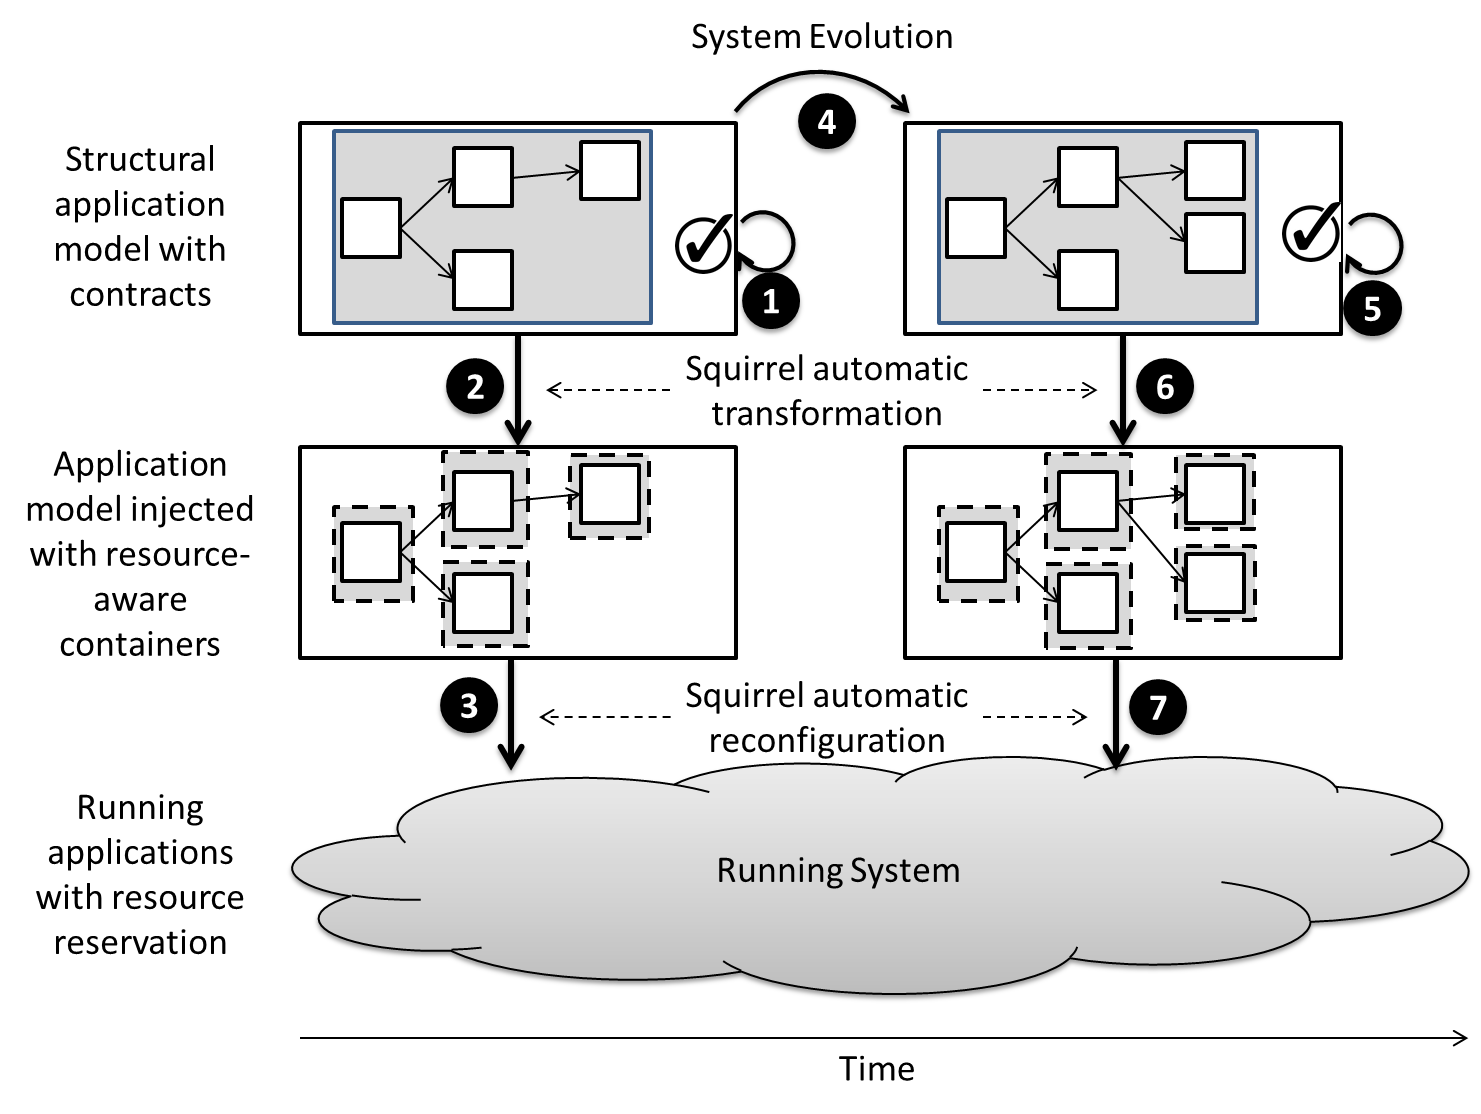
\includegraphics[width=0.7\textwidth]{chapter4/figures/globalOverview.png}
\caption{Squirrel approach for resources reservation} \label{fig:Overview}
\vspace{-0.5cm}
\end{figure}	

As illustrated in figure~\ref{fig:Overview}, Squirrel follows an automatic process to manage resources.
Squirrel receives an application's model, enhanced with contracts on resource reservation. 
Squirrel performs admission control to check the validity of the contracts on resource usage with respect to the available resources in the execution environment.
If the contracts are consistent with available resources, the process continues, if not, the application's model is refused.
Then, as depicted by arrow 2, Squirrel automatically transforms components or the configuration/architecture model by isolating components in resource-aware containers that can be finely configured to decrease the resource management overhead.
Finally, as depicted by arrow 3, Squirrel reconfigures the running system.
When the application evolves (arrow 4), 
%Squirrel automatically adapts the system while preserving resource reservation properties by applying the whole process on the new model (arrow 5, 6 and 7).
Squirrel attempts to preserve resource reservation properties while processing the new model (arrow 5, 6 and 7).


\subsection{Describing resource management requirements}
Beugnard et al. discuss the extending Meyer's \textit{Design-By-Contract} idea to software components~\cite{Beugnard774917}.
They classify component contracts into four categories: syntactic (level 1), semantic (level 2), synchronization (level 3), and Quality of Service (level 4).
%They explain that component contracts have to deal with concerns that they classified into 
%Fifteen years later, many component-based frameworks provide contracts that are used to: 
%i) Describe the component features with all required contracts.
%ii) Select from all contracts those that are useful in the context of component use, and configure them.
%iii) Evaluate contracts and react accordingly.
%iv) Decide when to stop evaluating contracts. 
There is no de-facto standard to describe component contracts, but many domain specific interface description languages contain such metadata.
This chapter assumes that components have contracts to deal with resource reservation (level 4).
A contract in Squirrel defines component resource requirements written in terms of resource types, quotas and expected component usage.
\begin{itemize}
\item{\textbf{Definition 1}} A resource type indicates any class of computational resource that is useful to a component.
Its consumption must be susceptible to monitoring and reservation.
In this paper, we consider CPU, Memory, Network Bandwidth and IO Throughput.

\item{\textbf{Definition 2}} Expected component usage describes the expected number of external invocations of each method of the component interface.
In short, let $C$ be a component instance, then $\forall{I \in C_{Interfaces}}, \forall{M \in I_{methods}} \\ {EU}_{IM}$ is the number of expected invocations of method $M$, per second.

\end{itemize}

A \textbf{contract in Squirrel} is a set of tuples with the form $\langle RT, N, MU \rangle$ where $RT$ is a resource type, N the maximum amount of resources to reserve, and $MU$ is the measuring unit used for this resource type.
Optionally, Squirrel supports the definition of a set of tuples with the form $\langle I, M, {EU}_{IM} \rangle$ where $I$ is a component interface, $M$ is a method of the interface, and ${EU}_{IM}$ the expected usage.
Implementations of the Squirrel approach must provide a way to define contracts with these concepts.
%In section~\ref{sec:kevoree} 
We use a domain-specific language to describe contracts.

\subsection{Admission control} \label{sect:admissionControl}

Providing resource reservation in a component based framework requires checking if components' resource-aware contracts are compatible with the resources available in the execution environment.
%The platform provides a fixed amount of resources that constitute the pool of resources used by components.
By checking the availability of resources, the platform controls component admissions.

%To support this dynamism while managing resources, 
To support resource management at runtime, Squirrel takes into account two events: i) component deployment, and ii) component removal.
%These are common operations on any middleware; hence adding a notification for these events is straightforward.
Whenever the application is modified, the system automatically recalculates the aggregated resources required by the application and compares it to the available resources in the execution environment.
If the available resources are greater than those required by the application, the reconfiguration is accepted, else, the application model is refused and the reconfigurations are discarded.

%\subsection{Defining multiple variants of execution model}
%\todo{I couldn't finish this, so I'm writing my ideas}
%To support our approach, a middleware needs to support multiple ways of mapping component instances into system/runtime abstractions.
%Somehow, it means that it needs an extension point to describe a factory for creating component instances.
%I can see two ways of doing so, either the writer of the middleware provides many versions of execution model or she provides a mechanism to extends the semantic of a component instance and of component containers (Node).
%In Kevoree we achieved this easily because it is naturally extensible, we can define new Node Types, New Channel Type, and we can compose them.
%Moreover, we use Models@Runtime to easily change between variant of mappings (e.g., we receive a model where each component is executed as a Thread and sometime we transform the model in order to execute components as processes). 

\subsection{Mapping component-model concepts to system-level abstractions}

%To map component-model concepts to system-level abstractions that allow for resource management, Squirrel defines steps to perform either during the design/implementation of the platform or at deployment time.
Squirrel defines steps to map component-model concepts to system-level abstractions that allow for resource management. Mappings can be applied during the design and implementation of the framework, or at deployment-time.
During framework design/implementation, developers identify system abstractions that are suitable to represent each concept and implement the respective mappings.
As a second step, resource management methods for each abstraction are implemented and evaluated.
This evaluation is used to determine the management methods with lowest overhead for each pair of system abstraction and resource type.
Later on, at deployment-time, the platform selects a component-to-system mapping using optimization techniques and the data obtained at design-time.
In this section, we briefly explain each step.

As we have mentioned, components can be represented through different system abstractions. % in the runtime platform.
This requires \textit{identifying possible mappings from components to system-level abstractions}.
Mappings must respect the semantics of the component model, and %but for a resource-aware platform, 
must provide resource management capabilities.
A key problem is that different mappings have different non-functional properties, and optimizations are often needed to make the mappings attractive. % competitive.
Additionally, an extensible design of the component platform, where it is easy to accommodate new mappings, greatly facilitates the co-existence of different mappings to represent a component. 
The set $ \textit{SA} $ of system abstractions that are available to represent a concept, along with the recommended optimizations for each abstraction, are defined in this step.

During the design/implementation of the platform it is necessary to \textit{define methods to manage resources} for each pair of system abstraction and resource type.
Developers must devise resource management methods for each mapping
% and resource type, 
 and identify the least costly.
If we consider different abstractions and resource types, we can define the matrices $ M $ and $ C $ where
$ \forall{\textit{sa} \in \textit{SA}, \textit{rt} \in \textit{RT}} $ the values
$  M_{\textit{sa}, \textit{rt}} $ and $ C_{\textit{sa}, \textit{rt}} $ indicate the method that minimizes the cost of managing the resource $ \textit{rt} $ when the abstraction $ \textit{sa} $ is used to represent a component. %, and this minimum cost.
%\hl{In a simple setting, the cost of each pair could be calculated as the mean overhead produced by the management method when some benchmarks are executed.[IS THIS PHRASE NECESSARY?]}
We make two assumptions about the resource management mechanisms: i) mechanisms are always composable if they manage different resource types, and ii) the costs of any pair of management mechanisms are independent.

At deployment-time, \textit{the platform selects the mapping} to use for each component in the application. % to deploy.
To do so, the platform uses the information contained in the matrices $ M $ and $ C $, the set of possible optimizations for each mapping, and the resource requirements of the application.
At this stage, the only data needed regarding resource requirements is the type of resource.
%Using this data, it is possible to apply an optimization method to select the best mapping candidate.
Using this data allows selecting the best mapping candidate.
Although we only use a single cost matrix that contains the overhead of each management mechanism, we think it is easy to generalize the approach to handle multi-objective optimizations with more than one cost matrix.
Others refinement to evaluate the cost of a mapping are possible.
For instance, we can consider the cost of using a specific binding to connect two components that use a given mapping.
Finally, there are many optimization methods that can compute the mappings, we do not propose any particular method in the approach.
However, the results shown in section~\ref{sec:evaluation} suggest that very simple heuristics can lead to good performance. 
 

%\todo{Here we should talk about the heuristic. We are trying to optimize, so we need to choose a mapping for each component. We only have a partial information about each resource managment mechanism. that's why we cannot perform classic optimization and we relies on heuristics}
%\todo{A conclusion here}


\section{Tooling}\label{sec:dsl-implementation}

To validate our approach, we have implemented a tool chain to ease the definition of custom memory profilers for Java-based systems.~\footnote{Available at: \url{https://github.com/intigonzalez/heapexplorer\_language}}
These profilers can be executed in any JVM as long as it provides support for the JVMTI.

In this section, we present tools built to support the definition of memory profilers using our language; this is done by taking into account how engineers in different roles may interact with these tools and with the resultant profilers.
Indeed, in dealing with memory profilers, we have to take into consideration the two usual roles -- developers of profilers and their users; after all, profilers built using our language are themselves software abstractions.
A developer must know how the target domain-specific abstractions are represented atop the JVM, and she also must have a clear understanding of how our language is executed.
On the contrary, users only need to be aware of the interface provided by our framework, and the structure of the data collected by a profiler.
In the rest of this section, we discuss details that are important to these roles.

Additionally, we present low-level details regarding how the language is implemented atop of the JMVTI.
The decision of implementing our approach by relying on JVMTI has advantages and disadvantages.
On the one hand, the obvious advantage lies on the portability of this solution, which makes it more valuable from a practical point of view.
On the other hand, building profilers on top of the JVMTI, instead of directly modifying the JVM, impacts the performance of the generated profilers and, unfortunately, hinders (in extreme case it even prevents) the implementation of some language constructs.
Nonetheless, it is our belief that guarantying profilers' portability should be of maximum priority.
Moreover, in writing this implementation, we have found that the limitations in the JVMTI preventing the construction of better profilers can be overcome with, at most, a few additions to the API.


\subsection{Developers of domain-specific abstractions}

%\extracomment{FIX}{I am fixing this section, you can continue in Section~\ref{sec:dsl-tooling-users}}

In our vision, developers of software libraries and component frameworks, as well as software language engineers may use our approach to  define customized memory profilers for the abstractions they create.
This is, in addition to delivering artifacts such as libraries, source code, simulators, text editors for DSLs, and compilers for these DSLs; engineers would also ship profilers to simplify the use of these abstractions.
For instance, the developers of the Spring framework~\footnote{\url{https://spring.io/}} may create a set of specific profilers to reduce the cost of maintaining applications written using the framework.
These profilers can serve as both internal tools to help in the development of abstractions, and mechanisms allowing users to better use abstractions.

Figure~\ref{fig:dsl-tooling-developer} summarizes the viewpoint of developers of domain-specific abstractions.
To write a profiler, they use knowledge about the abstraction and the tool chain to generate the executable profiler. 
Our implementation of the language is built using Xtext~\cite{Eysholdt:2010:XIY:1869542.1869625}; it provides a textual editor that is able to handle the proposed concrete syntax.
This editor provides syntax highlighting, error detection during editing, auto-completion, and compilation to native Java agents written in \textit{C++}.

\begin{figure}
\centering
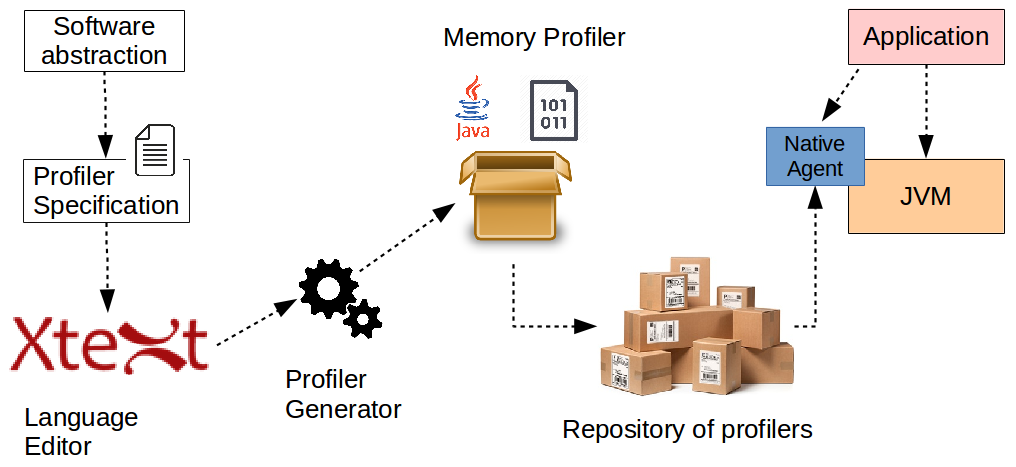
\includegraphics[scale=0.45]{./chapter6/fig/developer-profiler-view.png}
\caption{Viewpoint of developers. Memory profilers are built from the description of software abstractions.}\label{fig:dsl-tooling-developer}
\end{figure}

To perform low-level tasks related to memory profiling, we use \glslink{JVMTI}{JVMTI}~\footnote{\url{http://docs.oracle.com/javase/8/docs/platform/jvmti/jvmti.html}} and \glslink{JNI}{JNI}.
These APIs are used by both profilers and the core memory profiling library, so-called Native Agent in Figure~\ref{fig:dsl-tooling-developer}.
In this native agent, a \textit{plugins} system, which allows users to load/unload profiles without shutting down the JVM, is implemented.
Given a profiler definion, the compiler output is a package that contains a package with the native binary code for the profiler, and a Java library you can use to access the collected data using plain Java objects.

To reduce the overhead of profilers, developers must be aware of the details of the abstraction for which the profiler is being built, the semantic of our language, and the details of its implementation.
In particular, it is advisable reducing the usage of \textit{lists} and the evaluation of nested lambda expressions.
Likewise, heavily using the built-in rvalue \textit{objects} is specially discouraged because it can easily contains many elements.
It is also discouraged because, in order to reduce memory consumption, we rely on an iterator built on top of JVMTI operations that can be costly to use in terms of CPU time.

Finally, we added some built-in rvalues in this implementation because they are both useful in the context of Java and easy to obtain using the JVMTI.
These values are \textit{classes}, \textit{classloaders}, \textit{threads} and \textit{objects}; they are lists of anonymous built-in record types.
The relations among these types and their operations are depicted in Figure~\ref{fig:dsl-built-in-types}.

\begin{figure}
\centering
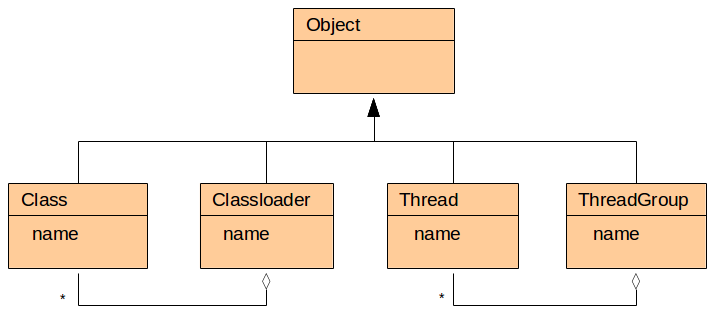
\includegraphics[scale=0.45]{./chapter6/fig/diagram-classes.png}
\caption{Viewpoint of developers. Memory profilers are built from the description of software abstractions.}\label{fig:dsl-built-in-types}
\end{figure}

%Indeed, the process of code generation is driven by the need of reducing the performance impact.
%In our implementation, we apply a set of platform dependent optimizations taking into account the profiler description.
%First, since a profiler does not always need built-in rvalues (e.g., \textit{threads}, \textit{threadgroups} and \textit{classes}, etc.), we selectively skip the construction of them.
%When possible, we also skip the construction of some structures (e.g., class of each object, its classloader, field names, etc.).

\subsection{Users of domain-specific abstractions} \label{sec:dsl-tooling-users}

We envision that a set of memory profilers can be shipped in addition to other ``classic'' deployment artifacts that users of a software abstraction receive. 
These profilers would support the use of the corresponding software abstraction.
For instance, an user who is relying on a new extension of the Xtend language to build a system, might use specific profilers written in our language to understand the memory consumption, and in general, the behavior of the system.

The generated profilers can be used in two different ways, either as development tools or as mechanisms to support resource awareness at runtime.
Due to the scope of this thesis, the reference implementation we provide is biased towards the second scenario, but it should be relatively simple to adapt it to support the software development process.
To access memory profilers, a JVM must be launched with a native Java agent loaded, and a library to collect profiling data in its classpath.
Once the application is running, it can trigger profiling by simple issuing a few method calls using the profiling API.
Figure~\ref{fig:user-profiling-library-view} illustrates the process of collecting memory profiles, the software components involved, and the APIs that must be used.
Observe how the profiling framework issues a call to a handler once it is done, a parameter contains the data computed.
These data are encoded in a \textit{list}, in which each elements correspond to the data computed for each identified structure in the heap.
%The problem is knowing the type and shape of each list element.

\begin{figure}[!b]
\centering
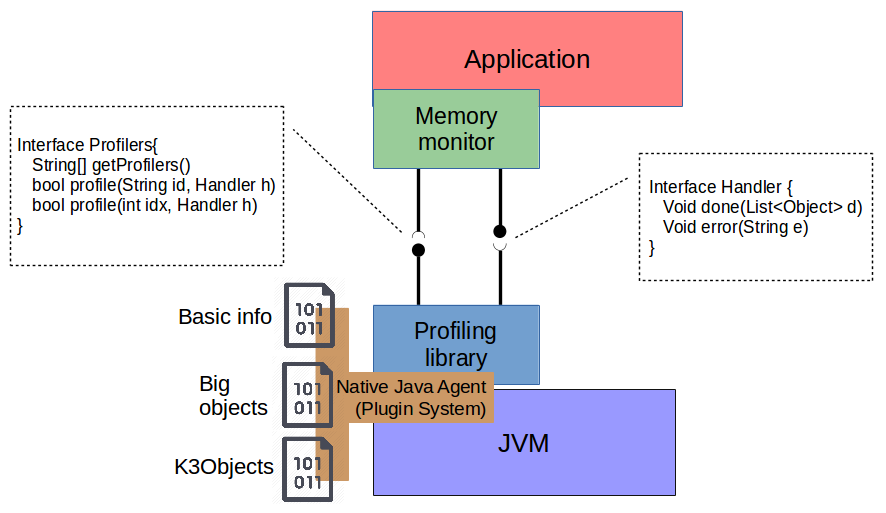
\includegraphics[scale=0.6]{./chapter6/fig/user-profiler-view.png}
\caption{Viewpoint of users. Memory profilers are black-boxes accessed through Java interfaces. Data collected is in the form of plain Java objects.}\label{fig:user-profiling-library-view}
\end{figure}

The output of a profiler is a list of Java objects containing the collected information; and the type of these objects depend on the profiler definition.
Indeed, as part of our implementation, the profiler generator creates a set of Java classes to represent the data collected in a form that is easy to digest at runtime by a Java application.
Once a profiler collects the information in an internal format, it populates a representation in Java using the Java Native Interface (JNI); the code to do so is also generated by the compiler of our language.
In Figure~\ref{fig:dsl-generated-java}, the classes generated for a profiler are shown.
Notice that a class is created for each \textit{record} declared, and also for each \textit{StructureType}.
It can be seen how `lists' are directly represented in Java by mean of generic Java lists.
The \textit{id} field in both \textit{MemoryProfile1} and \textit{MemoryProfile2} is the value used to parametrize each structure;
in this particular example, where two structures are identified, the value of \textit{MemoryProfile1.id} is ``lists'' and the value of \textit{MemoryProfile2.id} is ``otherObjects''.

Given the fact that the data computed by a profiler is returned as a list of objects, and their layout is unclear, the remaining problem is how to process such data; there are two options.
First, users can make the application code depend on the Java code created by the profiler generator.
In this way, your application has a new dependency, but you can profit from knowing at development time the types used in the code.
A second approach is using the reflection capabilities of Java to explore the data.
In the evaluation, we use such an approach to log the result of an arbitrary profiler, printing all the information it has computed.
Using reflection, it is also possible to build a user interface to explore the results in a customized way.  

\begin{figure}
\centering
\begin{minipage}[t]{0.60\linewidth}
\begin{lstlisting}[language=DSL2]
name "basic info" 

T : struct {
	classname : String
	size: int
}
create structeres for e:#["lists"]
using
	constructor
		initialObjects = #Object[]
		data1 = #T[];
	membership
		(this is String) or (this is Array)
	updates
		data1 = data.add(struct T { this.classname, this.size})
		
create structeres for e:#["otherObjects"]
using
	constructor
		initialObjects = #Object[]
		data2 = #T[];
	membership true
	updates
		data2 = data.add(struct T { this.classname, this.size})
\end{lstlisting}
\end{minipage}
\hspace{0.07\linewidth}
\begin{minipage}[t]{0.30\linewidth}
\begin{lstlisting}[language=java, frame=L, numbers=left,numberstyle=\color{black}\scriptsize]
class T {
	final String classname;
	final int size;
}

class MemoryProfile1 {
	final Object id;
	final List<T> data1;
}

class MemoryProfile2 {
	final Object id;
	final List<T> data2;
}
\end{lstlisting}
\end{minipage}
\caption{Representation of profiling data in Java, as users of profilers see it. Accessing these structures is useful to support resource awareness.} \label{fig:dsl-generated-java}
\end{figure}




%The process of code generation is driven by the need of reducing the performance impact.
%In general, there are two ways of optimizing the impact of the memory's analysis.
%First, we can apply platform dependent optimizations.
%The second option is to apply platform independent optimizations; for instance, simplifying the evaluation of each expression.
%In our implementation, we use both platform dependent and independent optimizations.
%
%A set of platform dependent optimizations we perform is related to the construction of the built-in values \textit{threads}, \textit{threadgroups}, \textit{classes}, etc. 
%Since not all memory analysis depends on such values, we selectively skip the construction of them.
%For instance, in listing~\ref{assertion} there is no need to compute any of such values as is also unnecessary to identified the class of each object.
%Extending this idea to other cases (e.g., class of each object, its classloader, field names, etc.) is straightforward.
%To implement these optimizations, we used a parametrized code template, so the code generate depends on the values of these parameters which we can tune to satisfy our needs.
%
%An other optimization we perform is related to the existence of collections as data type in our DSL.
%These collections can be potentially large, in particular, the \textit{objects} value is costly to compute and keep in memory.
%This fact combined with the usage of operations on collections such as \textit{map} and \textit{filter} may harm the performance of an analysis.
%That is why we devise two strategies to deal with collection values.
%User-defined and most built-in collections are kept in memory using linear space.
%On the contrary, we represent the built-in collection \textit{objects} as a generator.
%This representation is feasible because the mechanism provided by JVMTI to access the objects is based on callbacks.
%
%A last optimization is reducing the nodes of the graph that must be traversed
%As an illustration, we only produce code to explore primitive fields of each object, which are represented as leaf nodes in the graph, if there exist some expression accessing a field.
%
%As for platform independent optimizations, we mostly change the order in which boolean expressions are evaluated.
%We try to guarantee that subexpressions accessing collections and fields are evaluated as little as possible.
%
%The current implementation is limited in the number of optimization it applies.
%The main overhead reduction is achieved thanks to the execution model in which many paths of the graph are not traversed.
%Other benefits come from deciding at compilation time if some parts of the graph such as the leaf nodes must be explored or not.


\section{Evaluating performance of profilers}\label{sec:evaluation}
%\todo{Add research questions}

In this section we evaluate the implementation of our approach with several experiments.
To do so, we present a set of experiments to evaluate the performance overhead of executing different memory analysis.
A goal of this section is to show that our approach induces low overhead across different applications and types of analysis.
Since such analysis exhibit different levels of complexity, we cover a wide spectrum of use even if we are running the experiments with few types of analysis.
%We evaluate the performance of our DSL with several experiments:
 These experiments aim at answering the following research questions:
\begin{enumerate}
\item \textbf{RQ1. Does our approach produce profilers with lower overhead than state-of-the-art tools when used to perform many iterations of memory analysis at runtime?} To answer this question, we assess the overhead on total execution time produced by the periodic computation of a specific analysis.
In this experiment we measure and compare the overhead of our approach against the overhead produced by other solutions.
\item \textbf{RQ2. Is significant the difference between the time needed to execute a single analysis with our approach in comparison to previous solutions? }
In a second experiment, we measure the execution time needed to perform a single memory analysis step instead of focusing on the total application execution time.
\item \textbf{RQ3. Does the advantage of our approach remain for real applications? }
 Finally, we perform memory analysis on actual applications including \textit{Eclipse}, \textit{NetBean} and others to assess the overhead of profiling in ``real life'' scenarios. 
\end{enumerate}

In general, these experiments show that our DSL produces specific profilers with lower overhead for applications running in production environments than well-known memory profilers.

\subsection{Methodology and Setup}\label{sec:MethodologyAndSetup}
Our system is implemented on top of JVMTI, thus we compare our results using the HotSpot JVM version 1.7.0\_76, with a heap size of 2GiB for all the experiments.
Across this section we use Eclipse Memory Analyzer 1.4.0 (Eclipse MAT),  a production ready memory profiler, to perform several experiments.
We use  this tool in console user interface (CLI) mode that executes the desired analysis on a separate process.
In short, when performing a memory analysis on a JVM instance \textit{A}, we dump its heap and invoke Eclipse MAT in a separate JVM instance to collect profiling data.

We use DaCapo benchmarks version 2006-10-MR2~\cite{DaCapo:paper} with the large input size for the first experiment and with different input sizes in the second one.
In the third experiment we use a set of actual applications based on OSGi, these applications are listed in the relevant section~\footnote{Links are available at https://en.wikipedia.org/wiki/OSGi}.
Although the details are specific to each experiment, in general each measurement presented is the average of several runs under the same conditions.

To obtain comparable and reproducible results, we used the same hardware across all experiments: a 2.90GHz Intel(R) i7-3520M processor, running Linux with a 64 bit kernel version 3.17.3 and 8GiB of system memory.

\subsection{Impact of Analysis on the Total Execution Time}

In this experiment we assess the overhead of our approach on the total execution time of applications.
To do so, we compare the execution time reported by the DaCapo benchmarks without any kind of memory analysis against the execution time when our DSL is used to perform the analysis in listing~\ref{kevoreeaccounting}.
In addition, we check how our approach behaves in comparison to other approaches for memory analysis.
In this case, the analysis finds the number of objects and their total size when threads are used as only roots to traverse the graph of live objects.

The experiment was configured as follows: within a JVM instance we wrap the execution of the DaCapo Benchmark.
Each DaCapo test is configured to execute 20 warm-up iterations before the final test execution.
This number of warm-ups is used to guarantee a long enough execution time.
A separate thread periodically performs a \textit{memory consumption monitoring step} every 2 seconds by using one of the methods we want to compare: \textit{No analysis}, \textit{Handwritten JVMTI}, \textit{Our approach}, \textit{Heap Dump + Eclipse MAT}.

In addition to our approach, we implemented a \textit{handwritten JVMTI} agent as well as an Eclipse MAT's  extension to collect the same data.
In the \textit{handwritten JVMTI}, we traverse all the references in the graph of live objects starting on the threads, during this process the JVM is fully halted impacting the total application's execution time.
The \textit{Heap Dump + Eclipse MAT} solution uses the approach described in section~\ref{sec:MethodologyAndSetup}; when an analysis is required, the JVM dumps the heap and executes Eclipse MAT on a separate process in CLI mode.

\begin{figure}[b]
\centering
\begin{tikzpicture}
\begin{axis}[ybar=0pt, legend style={at={(0.72,1)},
every axis legend/.append style={nodes={right}},
anchor=north,legend columns=1, font=\tiny},
ylabel={Overhead (\%)},
y label style={at={(0.06, 0.5)}},
scaled y ticks = false,
      y tick label style={/pgf/number format/fixed,
      /pgf/number format/1000 sep = \thinspace % Optional if you want to replace comma as the 1000 separator 
      },
xtick=data,ymin=0,
width = \columnwidth,
height = 4.2cm,
bar width = 5,
x tick label style={rotate=45,anchor=east, font=\small},
 axis lines*=left, % Don't display the top and right lines
 symbolic x coords={antlr,fop,hsqldb,jython,chart,luindex,xalan,lusearch, pmd, eclipse}
]
\addplot coordinates 
	{(antlr,3.9781514264) (fop,4.605707750) (hsqldb,29.2388250106) (jython,1.3401924419) (chart,2.9126870659) (luindex,7.4126736676)
	(xalan,3.5175679043) (lusearch,2.1071653048) (pmd,2.1071653048) (eclipse,13.2922104461) };
\addplot coordinates 
	{(antlr,4.6792415918) (fop,10.920169369) (hsqldb,33.4078193658) (jython,7.3669103815) (chart,10.0961181121) (luindex,5.8949045922) 
	(xalan,10.6595492114) (lusearch,8.8185623499) (pmd,11.7847827707) (eclipse,15.7219232736)};
\addplot coordinates 
	{(antlr,28.7859273871) (fop,23.7271506764) (hsqldb,46.0448750552) (jython,32.4395399802) (chart,44.6349538836) (luindex,31.9874187461) 
	(xalan,37.7533619117) (lusearch,12.9664891096) (pmd,33.9112866499) (eclipse,32.6863711858)};
\legend{Handwritten JVMTI, Our approach, Heap Dump + Eclipse MAT}
\end{axis}
\end{tikzpicture}
\caption{Overhead on execution time compared to the execution without memory analysis for different tests in the DaCapo Benchmark\label{fig:evaluationTotalTime}}
\end{figure}

In this experiment, we measure the total time needed to complete the 20 warm-up iterations plus the time required to execute the final test.
We repeat this process 10 times for each test in the DaCapo benchmark suite and take the average as final measurement.
First, it is useful to highlight how many time the analysis is performed.
As we mentioned, the analysis runs periodically, so the number of executions depends on the benchmark and the overhead produced by the analysis method.
With our approach, the analysis is executed a minimum of 10 times for \textit{fop} and a maximum of  366 times for \textit{eclipse}.
Figure~\ref{fig:evaluationTotalTime} depicts the overhead in the total execution time of DaCapo tests for different analysis strategies.
The values are shown as the percentage with respect to the baseline which in this case is obtained when \textit{no analysis} is executed.
It is noteworthy that our approach performs close to the handwritten solution.
Moreover, our solution outperforms the \textit{Heap Dump + Eclipse MAT} approach even when the latter is executing mostly on a separate process without halting the JVM during the analysis.

\subsection{Comparing Analysis Time for an Assertion}

In the previous section we show the overhead on the total execution time for different analysis mechanisms.
However, these mechanisms are not executed under the same conditions.
For instance, as we mention in section~\ref{sec:implementation} our implementation suspends the execution of the application while it performs the analysis.
On the contrary, the \textit{Heap Dump + Eclipse MAT} approach only suspends the application while dumping the heap, but the analysis is done in a separate process, so it likely runs in parallel.
Therefore, in this experiment we compare only the analysis time using well-known macro-benchmarks.
Since the analysis time depends on the number of objects visited during the computation, we assess in this experiment the behavior of our approach with a memory analysis that must iterate over all objects to complete.
For the same reason, we repeat the analysis with varying input size, which implies different number of objects in memory, to the macro-benchmarks.

The \textbf{assertion} used in this experiment checks \textbf{if there exist an instance of a specific class in the heap}.
The following listing shows how to implement such an assertion in our DSL.
The \textit{StructureType} definition guarantees that all objects are visited by defining the \textit{membership} property as the \textit{true} constant.
\begin{lstlisting}[escapeinside={(*}{*)},
%caption=Detecting if there exists an instance of a specific class, 
%label=lst:SimpleAssertion,
%float=!h,
frame=none, 
language=DSL2,numbers=left,
numbersep=2pt,
numberstyle=\color{black}\scriptsize,]
create structure foreach e:#["jvm"] using
   constructor
      initialObjects = #[]
      exists = false
   membership  true
   updates
      exists = exists or (this is UnusedClass)
\end{lstlisting}

\begin{figure*}[!ht]
 \centering
 \begin{minipage}[t]{0.45\linewidth}
 \centering
\begin{tikzpicture}
\begin{axis}[
ybar=0pt, 
legend style={at={(0.72,1)},
every axis legend/.append style={nodes={right}},
anchor=north,legend columns=1, font=\tiny},
ylabel={Analysis Time (sec)},
y label style={at={(0.06, 0.5)}},
scaled y ticks = false,
      y tick label style={/pgf/number format/fixed,
      /pgf/number format/1000 sep = \thinspace % Optional if you want to replace comma as the 1000 separator 
      },
xtick=data,ymin=0,
width = \columnwidth,
height = 4.2cm,
bar width = 5,
x tick label style={rotate=45,anchor=east, font=\small},
 axis lines*=left, % Don't display the top and right lines
 symbolic x coords={antlr,fop,hsqldb,jython,chart,luindex,xalan,lusearch, pmd, eclipse}
]
\addplot coordinates 
	{(antlr,1.9781514264) (fop,1.605707750) (hsqldb,2.2388250106) (jython,1.3401924419) (chart,2.9126870659) (luindex,1.4126736676)
	(xalan,1.5175679043) (lusearch,2.1071653048) (pmd,1.1071653048) (eclipse,3.2922104461) };
\addplot coordinates 
	{(antlr,2.2781514264) (fop,1.805707750) (hsqldb,2.5388250106) (jython,1.6401924419) (chart,3.2126870659) (luindex,1.6126736676)
		(xalan,1.7175679043) (lusearch,2.4071653048) (pmd,1.3071653048) (eclipse,3.5922104461) };
\addplot coordinates 
	{(antlr,2.9781514264) (fop,2.605707750) (hsqldb,3.2388250106) (jython,2.3401924419) (chart,3.9126870659) (luindex,2.4126736676)
		(xalan,2.5175679043) (lusearch,3.1071653048) (pmd,2.1071653048) (eclipse,4.2922104461) };
%\legend{Handwritten JVMTI, Our approach, Heap Dump + Eclipse MAT}
\end{axis}
\end{tikzpicture}
\caption{Analysis time with default input size\label{fig:analysisTimeDefaultSize}}
\end{minipage}
 \begin{minipage}[t]{0.45\linewidth}
 \centering
\begin{tikzpicture}
\begin{axis}[ybar=0pt, legend style={at={(0.23,1.13)},
every axis legend/.append style={nodes={right}},
anchor=north,legend columns=1, font=\tiny},
ylabel={Analysis Time (sec)},
y label style={at={(0.06, 0.5)}},
scaled y ticks = false,
      y tick label style={/pgf/number format/fixed,
      /pgf/number format/1000 sep = \thinspace % Optional if you want to replace comma as the 1000 separator 
      },
xtick=data,ymin=0,
width = \columnwidth,
height = 4.2cm,
bar width = 5,
x tick label style={rotate=45,anchor=east, font=\small},
 axis lines*=left, % Don't display the top and right lines
 symbolic x coords={antlr,fop,hsqldb,jython,chart,luindex,xalan,lusearch, pmd, eclipse}
]
\addplot coordinates 
	{(antlr,2.3781514264) (fop,1.905707750) (hsqldb,2.7388250106) (jython,1.8401924419) (chart,3.1126870659) (luindex,1.6126736676)
	(xalan,1.7175679043) (lusearch,2.2171653048) (pmd,1.3171653048) (eclipse,3.3822104461) };
\addplot coordinates 
	{(antlr,2.5781514264) (fop,1.945707750) (hsqldb, 2.7818250106) (jython,2.0401924419) (chart,3.6326870659) (luindex,1.912632376)
		(xalan,1.9375679043) (lusearch,2.4071653048) (pmd,1.3999716530) (eclipse,3.7922104461) };
\addplot coordinates 
	{(antlr,3.9781514264) (fop,3.605707750) (hsqldb,4.2388250106) (jython,3.3401924419) (chart,4.9126870659) (luindex,3.4126736676)
		(xalan,3.5175679043) (lusearch,4.1071653048) (pmd,3.1071653048) (eclipse,5.2922104461) };
\legend{Handwritten JVMTI, Our approach, Heap Dump + Eclipse MAT}
\end{axis}
\end{tikzpicture}
\caption{Analysis time with large input size\label{fig:analysisTimeLargeSize}}
 \end{minipage}
\hspace{1cm}
\end{figure*}

The setting of the experiment is as follow.
The DaCapo benchmark suite is used with two different input sizes, default and large.
Before the final test, twenty warm-ups are executed in order to ensure long enough execution time.
A separate thread periodically checks the assertion and records the analysis time.
The average analysis time along the complete execution of a benchmark (i.e., xalan, fop, ...) is used as data point.
Ten of these data points are obtained through repetition of the previous step and used as final measurement for a pair of benchmark and analysis approach.
As in the previous experiment, we use a handwritten JVMTI agents and an Eclipse MAT extension to check the assertion with those tools.

Figures~\ref{fig:analysisTimeDefaultSize} and~\ref{fig:analysisTimeLargeSize} present the results of the experiments.
In both cases, default and large input size, our DSL is in between the handwritten JVMTI agent and the Eclipse MAT approach.
In comparison to Eclipse MAT, our approach on average reduces the analysis time in 25\% and 39\% for default and large input size respectively.
As expected, the analysis time increases with the number of objects, the slowdown shown between default and large input size is of 8.42\%.

\subsection{Analysis Time in Real Scenarios}
To evaluate the overhead of our approach in actual applications, 
we compute the memory consumption of bundles in real OSGi-based systems.
Since OSGi is a widely used framework, we chose applications built on top of OSGi or supporting it.
The custom profiler definition is based on the idea that bundle consumption is the consumption of a Java classloader.
Such a strategy is common when measuring memory consumption for Java-based component frameworks because modules are often isolated and represented through classloaders.
The complete profiler's definition is shown below:
\begin{lstlisting}[escapeinside={(*}{*)},
%caption=Calculating the consumption of top components,
%label=topcomponents,
%float=!h, 
frame=none,
numbers=left,
numbersep=2pt,
numberstyle=\color{black}\scriptsize,
language=DSL2]
create structure foreach e:classloaders using
  constructor
    initialObjects = #[e]
    nbSize = 0
  membership  (this in None) and 
    ((ref_kind = root and this.class.classloader in this_structure) or
	(ref_kind (*$\neq$*) root and referrer in this_structure))
  updates
    nbSize = nbSize + this.size
\end{lstlisting}

This experiment aims at evaluating the analysis time for each application using our approach and \textit{Heap Dump + Eclipse MAT}.
In this experiment, each application is executed. Once it is initialized, the memory analysis is performed and its execution time measured.
This process is repeated ten times for each application and analysis approach in order to use the average as final measurement.
We use \textit{Heap Dump + Eclipse MAT}  to compute the memory retained for top level classloaders using  a standard analysis named \textit{top components} reports. 

To execute the memory analysis from within the applications, we implemented extensions for each application (e.g., an Eclipse plugin, a NetBean module).
These extensions are in charge of triggering the analysis.
It was necessary because in our approach the analysis must be executed by the JVM that is being profiled.
In this experiment, we perform the analysis on the following systems: Eclipse Luna~\cite{luna}, NetBeans 8.0\cite{netbeans}, dotCMS 3.1~\cite{dotcms}, Cytoscape 3.2.1~\cite{cytoscape}, Glassfish 4.1~\cite{glassfish},  Liferay 6.2.2~\cite{liferay}, WildFly 8.2~\cite{wildfly}.

Figure~\ref{fig:analysisTime} presents the analysis time for several applications and two analysis approaches.
Our DSL outperforms other solutions for all applications.
The gain is 3x-19x with an average of 8x.
This gain is due to two factors.
First the Eclipse MAT solution invests some time parsing the dump file and creating the internal indexes to accelerate queries' response time.
Second, the \textit{top components} report in Eclipse MAT can only be implemented using its query language in terms of the function \textit{retainedHeapSize} which calculates the amount of memory retained for a given object.
Since this function is costly to compute, Eclipse MAT spends a considerable amount of the time on it while building the \textit{top components} report. The evaluation code is available online~\footnote{https://github.com/intigonzalez/heapexplorer\_language}.

\begin{figure}[!b]
\centering
\begin{tikzpicture}
\begin{axis}[ybar=0pt, legend style={at={(0.72,1)},
every axis legend/.append style={nodes={right}},
anchor=north,legend columns=1, font=\tiny},
ylabel={Analysis Time (sec)},
y label style={at={(0.06, 0.5)}},
scaled y ticks = false,
      y tick label style={/pgf/number format/fixed,
      /pgf/number format/1000 sep = \thinspace % Optional if you want to replace comma as the 1000 separator 
      },
xtick=data,ymin=0,
width = \columnwidth,
height = 4.2cm,
bar width = 5,
x tick label style={rotate=45,anchor=east, font=\small},
 axis lines*=left, % Don't display the top and right lines
 symbolic x coords={Eclipse Luna, NetBean 8.0, dotCMS 3.1,Cytoscape 3.2.1,Glassfish 4.1, Liferay 6.2.2, WildFly 8.2}
]
\addplot coordinates 
	{(Eclipse Luna,3.9781514264) (NetBean 8.0, 4.605707750) (dotCMS 3.1, 9.2388250106) (Cytoscape 3.2.1, 1.3401924419) (Glassfish 4.1, 2.9126870659) (Liferay 6.2.2,4.9126870659) (WildFly 8.2, 3.9126870659) };
\addplot coordinates 
	{(Eclipse Luna,42.133233423) (NetBean 8.0,38.388906289) (dotCMS 3.1,30.9167577408) (Cytoscape 3.2.1,25.99) (Glassfish 4.1, 18.46) (Liferay 6.2.2, 28.9126870659) (WildFly 8.2, 19.9126870659)};
\legend{Our Approach, Heap Dump + Eclipse MAT}
\end{axis}
\end{tikzpicture}
\caption{Analysis time for real applications. It shows the time needed to compute an analysis just once. The analysis aims at finding the consumption of the top components\label{fig:analysisTime}}
\end{figure}

%The results shown in figure~\ref{fig:evaluation} confirm the conclusions already discussed.
%Furthermore, they gave an initial estimation of the baseline overhead we can expect when the DSL approach is used.



\section{Related Work} \label{sec:related-works}
%\todo{Walter + inti + olivier}

%Lots of approaches~\cite{Oreizy:2008:RSA:1370175.1370181} demonstrate the benefits of component-based systems to support runtime adaptation in order to handle Quality of Service (QoS) reservation or QoS improvement.
The Squirrel approach is mainly related to i) component isolation for fine-grained resource management, ii) efficient communication between containers, and iii) efficient container initialisation. We discuss the related works for these topics. 

%\fancynote{Inti}{I am not writing the story. I am just listing related papers. That's what you asked me last time}
% a paragrapth to talk about resource monitoring, I-JVM, Charles University (Binder), Other, the paper by Kouter
	

\textbf{Component isolation for fine-grained resource management.}
%A first solution to support resource aware component management is to use monitoring. 
In the Java world, several approaches describe the use of monitoring to achieve resource-aware programming~\cite{Guidec:2003:JMP,Maurel:2012:AME:2304736.2304763,Moreau:2005:RAP}.
In \cite{binder_portable_2006,Hulaas:2008:PTL} the authors propose mechanisms based on bytecode instrumentation to monitor CPU and memory consumption.
%The instrumentation consists in adding calls to a resource monitoring agent during class loading.
Yet, instrumentation introduces high overhead and the monitoring framework contaminates the measurements
%contaminates the 
%Furthermore, the measurements are contaminated by the monitoring framework
because it is performed in the context of the monitored JVM.
%To avoid such a negative effect, the authors of \cite{Marek:2013:SRC} introduce ShadowVM. This framework delegates monitoring tasks to separate processes.
%However, the required communication also produces additional CPU overhead.
Geoffray et al.~\cite{Geoffray:2009:I-JVM} introduce a modification to the garbage collector to achieve lightweight memory accounting for OSGi containers.
%This modification has lower overhead than using instrumentation. 
Our work shows how we can automatically isolate components with resource contracts with low overhead through the execution of components on isolated system containers.

% about communication
\textbf{Efficient Inter-Container/Process communication}.
In~\cite{Unrau:708530}, the authors devise mechanisms for IPC based on building a queue in shared memory. As in our case, these solutions perform two data copies.
Nonetheless, the authors do not consider the problem of sending messages to multiple targets, which is a concern for us.
In Android, Binder is used to support IPC. 
Although it is a single-copy mechanism, its common usage in applications still requires two copies due to marshaling.
The limitations of the built-in serialization in Java are described by Bouchenak et al.~\cite{bouchenak2003techniques}.
Protocol buffers \cite{protobuf} provides an Interface Definition Language to generate RPC artifacts in different languages. 
Although the performance is good, it makes mandatory the use of an IDL, which is often a burden for engineers.
We propose to use a combination of shared-memory-based channels and a high-performance serialization library to marshal POJOs.


% about initialization time, talk also about VM
\textbf{Fast container initialization.} 
%Several approaches show the need to improve the initialisation time of containers or VMs. 
A goal of the MVM~\cite{czajkowski2012multitasking} is to provide fast initialization of new Java Applications.
By sharing the standard library among JVM instances, the authors reduce initialization time for new applications the bootstrap classes are already loaded.
However, the MVM is a non-trivial modification to a JVM and its current implementation does not support the latest version of the JDK~\cite{czajkowski2012multitasking}. 
Android \cite{Kalkov:2012:REA:2388936.2388955,Nagata:2013:MIA:2569436.2570296} uses a process, named Zygote, that loads the standard classes and is a sort of pre-initialized Dalvik VM.
Zygote receives demands to create copies of itself that mutate into Dalvik VMs. %executing applications.
%The approach leverages the \textit{fork} system-call to clone a process and it also uses copy-on-write to reduce memory consumption and initialization time. 
%On the contrary, 
We use an external tool, CRIU, to speed-up the creation of new JVMs because current JVM implementations do not provide built-in facilities for doing so.

%\paragraph{Practical considerations \todo{Move to perspectives}}
%A component does not execute on top of a flat operating system process but on top of a managed runtime environment, the JVM.
%As a consequence, we devote resources to the component but also to the middleware.
%Due to the presence of the garbage collector, we do not know the exact amount of memory new \textit{JVM nodes} should be assigned with.
%In fact, we can only state that the reserved memory must equal the component reservation plus the middleware requirement plus any amount that allows an efficient behavior %of the garbage collector.
%Chances are that any prediction will overestimate the real consumption, leading to the problem of wasting resources due to internal fragmentation.

\section{Conclusion} \label{sec:squirrel-conclusions}

%\enlargethispage{0.3cm}

In this chapter, we advocate for a methodology to provide resource management capabilities to dynamic component-based frameworks.
This methodology and its implementation, Squirrel, propose choosing component-to-system mappings at deployment time for better resource management.
This strategy is performed automatically by checking the resource availability and transforming the application's structure to run the application on resource-aware containers.
Containers describe how to map components to system abstractions
%in ways that reduce the cost of resource management.
allowing for different trade-offs in resource management.

The implementation we present is able to manage CPU, I/O and memory, and provide performance analyses and a comparison of different design decisions.
The experiments show that choosing the right component-to-system mappings at deployment-time reduces CPU overhead and/or memory use.
They also highlight that optimizing mappings is essential to reducing isolation and communication overhead to acceptable levels.

The approach proposed in this chapter contributes to answer the research question \textit{RQ2} (\textit{How can we choose what mechanisms must be used to guarantee resource reservation with low overhead for each component?}).
Instead of selecting a fixed resource reservation mechanism for all components, we delays this selection until deployment time when we know exactly what resources a component require.
At this point, we can specialize the approach used to reserve resources in such a way that performance overhead is kept at a low level.



%\begin{equation}
%  \psi (u) = \int_{o}^{T} \left[\frac{1}{2}
%  \left(\Lambda_{o}^{-1} u,u\right) + N^{\ast} (-u)\right] dt \;  .
%\end{equation}

%\subsubsection*{Acknowledgments.} The heading should be treated as a
%subsubsection heading and should not be assigned a number.

\bibliographystyle{abbrv}
\bibliography{biblio}  % sigproc.bib is the name of the Bibliography in this case

%\section{Checklist of Items to be Sent to Volume Editors}
%Here is a checklist of everything the volume editor requires from you:

%\begin{itemize}
%\settowidth{\leftmargin}{{\Large$\square$}}\advance\leftmargin\labelsep
%\itemsep8pt\relax
%\renewcommand\labelitemi{{\lower1.5pt\hbox{\Large$\square$}}}

%\item The final \LaTeX{} source files
%\item A final PDF file
%\item A copyright form, signed by one author on behalf of all of the
%authors of the paper.
%\item A readme giving the name and email address of the
%corresponding author.
%\end{itemize}
\end{document}
